% 評価結果


% 消費電力:USBテスタ(AVHzYct-3)を使用して測定し,消費電力を確認.
% 安定性:波形データから安定性を評価し,機器の安定した計測・データ送信の有無を確認.
% 稼働時間:Webシステムにデータが表示されなくなるまでの時間を測定.
% 精度:市販のTesto 405iと比較して,開発した測定機器の精度を確認.
% 寸法:各機器のサイズ比較.
% 価格:各機器のコストパフォーマンスを評価.
% 他社サービスとの比較:他社の製品やサービス(Testo 405i,Wi-Musu,Gill WindObserver 65など)との比較.




\section{概要}

本章では,第5章までに述べた測定方式および試作した小型 CO$_2$ 測定デバイスを用いて実施した各種測定実験の結果を示し,携帯型測定デバイスとしての有効性および実用性について評価を行うことを目的とする.特に,本研究で試作した携帯型 CO$_2$ 測定デバイスが,据え置き型 CO$_2$ 測定機器と比較して,環境中の CO$_2$ 濃度変化を適切に捉えることができるか,また実際の生活環境や移動環境において利用可能であるかに着目して検討を行う.はじめに,実環境における測定に先立ち,測定機器の基礎特性確認を行う.具体的には,CO$_2$ 測定機器の選定ガイドラインに基づき,アルコールおよび呼気に対する応答特性を評価し,本研究で使用した測定デバイスが CO$_2$ 濃度測定を目的とした機器として適切な特性を有しているかを確認する.この結果を踏まえ,以降の実環境測定において本測定デバイスを用いる妥当性を示す.次に,据え置き型 CO$_2$ 測定機器との比較測定を行い,両者を同一環境下に設置した際の CO$_2$ 濃度の時間変化を比較する.長時間にわたる測定結果を基に,携帯型測定デバイスが据え置き型測定機器と同様の CO$_2$ 濃度変化の傾向を捉えられているかを評価し,携帯型デバイスとしての測定信頼性について検討する.
さらに,空間的に CO$_2$ 濃度のばらつきが生じる環境として,福岡県赤村に設置されたドームハウスを対象に測定を行う.ドームハウス内には,床付近から天井付近にかけて多数の据え置き型 CO$_2$ 測定機器を設置し,高さ方向における CO$_2$ 濃度分布を把握する.その上で,携帯型 CO$_2$ 測定デバイスを用いた測定結果と比較し,空間内における相対的な CO$_2$ 濃度分布や換気が不十分な領域を,携帯型デバイス単体で把握できるかを評価する.
また,実際の生活環境および移動環境における測定例として,電車内における CO$_2$ 濃度の時間変化を測定する.異なる位置において測定を行うことで,車内における換気状況や混雑状況の変化が CO$_2$ 濃度に与える影響を明らかにし,携帯型測定デバイスが移動環境においても有効に機能するかを検討する.
加えて,本章では測定機器の省電力性能および小型化に関する評価を行う.通信方式の異なる測定機器を用いて,バッテリ駆動時の稼働時間を比較することで,通信方式が消費電力に与える影響を明らかにする.また,段階的に試作した測定機器1~4の外形寸法を整理し,小型化の進展について定量的に評価することで,携帯型 CO$_2$ 測定デバイスとしての実用性を検討する.
以上の評価を通じて,本研究で提案する携帯型 CO$_2$ 測定デバイスが,据え置き型測定機器と同様に CO$_2$ 濃度変化を把握可能であり,かつ日常生活環境や移動環境において利用可能な測定手段であることを示す.以下では,各測定環境における測定結果および評価について,順に詳述する.

\subsection{測定機器の基礎特性確認結果および評価}

図\ref{fig:alcohol_breath}に,アルコールおよび呼気に対するCO$_2$濃度の測定結果を示す.測定開始から20分後に,アルコールを入れたコップおよびアルコールを浸したティッシュを測定デバイス近傍に設置したが,この期間においてCO$_2$濃度に顕著な変化は認められなかった.

一方,測定開始から40分後に,測定デバイスに向けて1分間連続して呼気を吹きかけた際には,CO$_2$濃度が急激に上昇する挙動が確認された.この上昇は呼気付与の直後に生じており,呼気中に含まれるCO$_2$に対して測定デバイスが応答していることを示している.

以上の結果から,本研究で使用したCO$_2$測定デバイスは,アルコール蒸気に対しては反応せず,呼気中のCO$_2$に対しては明確に反応する挙動を示した.この挙動は,CO$_2$測定機器の選定ガイドラインに示される基本的な応答特性と整合しており,本デバイスがCO$_2$濃度測定を目的とした測定機器として適切な特性を有していることが確認できる.したがって,本研究では以降の実環境測定において,本測定デバイスを用いてCO$_2$濃度の測定を行うこととした.

\begin{figure}[H]
\centering
\includegraphics[width=0.9\linewidth]{./figures/alcohol}
\caption{
アルコール,呼気への反応結果
}
\label{fig:alcohol_breath}
\end{figure}

\section{据え置き型測定機器との測定値比較}

本節では,据え置き型CO$_2$測定機器と,本研究で試作した携帯型CO$_2$測定デバイスを同一環境下に設置し,両者の測定値の時間変化を比較した結果について述べる.測定は13時30分から24時30分までの約11時間にわたり実施し,両測定機器ともに5分間隔でCO$_2$濃度を測定した.

図\ref{fig:fixed_vs_portable}に,据え置き型測定機器および携帯型測定機器によるCO$_2$濃度の時間変化を示す.測定開始直後には,両測定機器ともに高いCO$_2$濃度を示しており,その後,時間の経過とともにCO$_2$濃度が低下する傾向が確認された.なお,測定開始直後に観測された高いCO$_2$濃度は,測定機器設置作業時に呼気が測定機器近傍にかかったことによる一時的な影響であると考えられる.この低下傾向は,両測定機器においてほぼ同時に観測されている.また,18時30分頃には,両測定機器の測定値においてCO$_2$濃度の上昇が確認され,その後再び低下する挙動が見られた.このようなCO$_2$濃度の増減のタイミングは,据え置き型測定機器と携帯型測定機器の間で概ね一致しており,両者が同一環境におけるCO$_2$濃度変化を捉えていることが分かる.

一方で,携帯型測定機器の測定値は,据え置き型測定機器と比較して一部の時間帯においてわずかな差が見られる.これは,測定機器の設置位置や個体差,応答特性の違いによる影響であると考えられる.しかしながら,CO$_2$濃度の上昇および低下といった時間変化の傾向は両者で概ね一致している.

以上の結果から,本研究で試作した携帯型CO$_2$測定デバイスは,据え置き型CO$_2$測定機器と同様のCO$_2$濃度変化の傾向を示すことが確認できた.このことから,携帯型測定機器は同一環境下においてCO$_2$濃度の時間的な変化を把握する用途において,据え置き型測定機器と同等の情報を取得可能であると考えられる.

\begin{figure}[H]
\centering
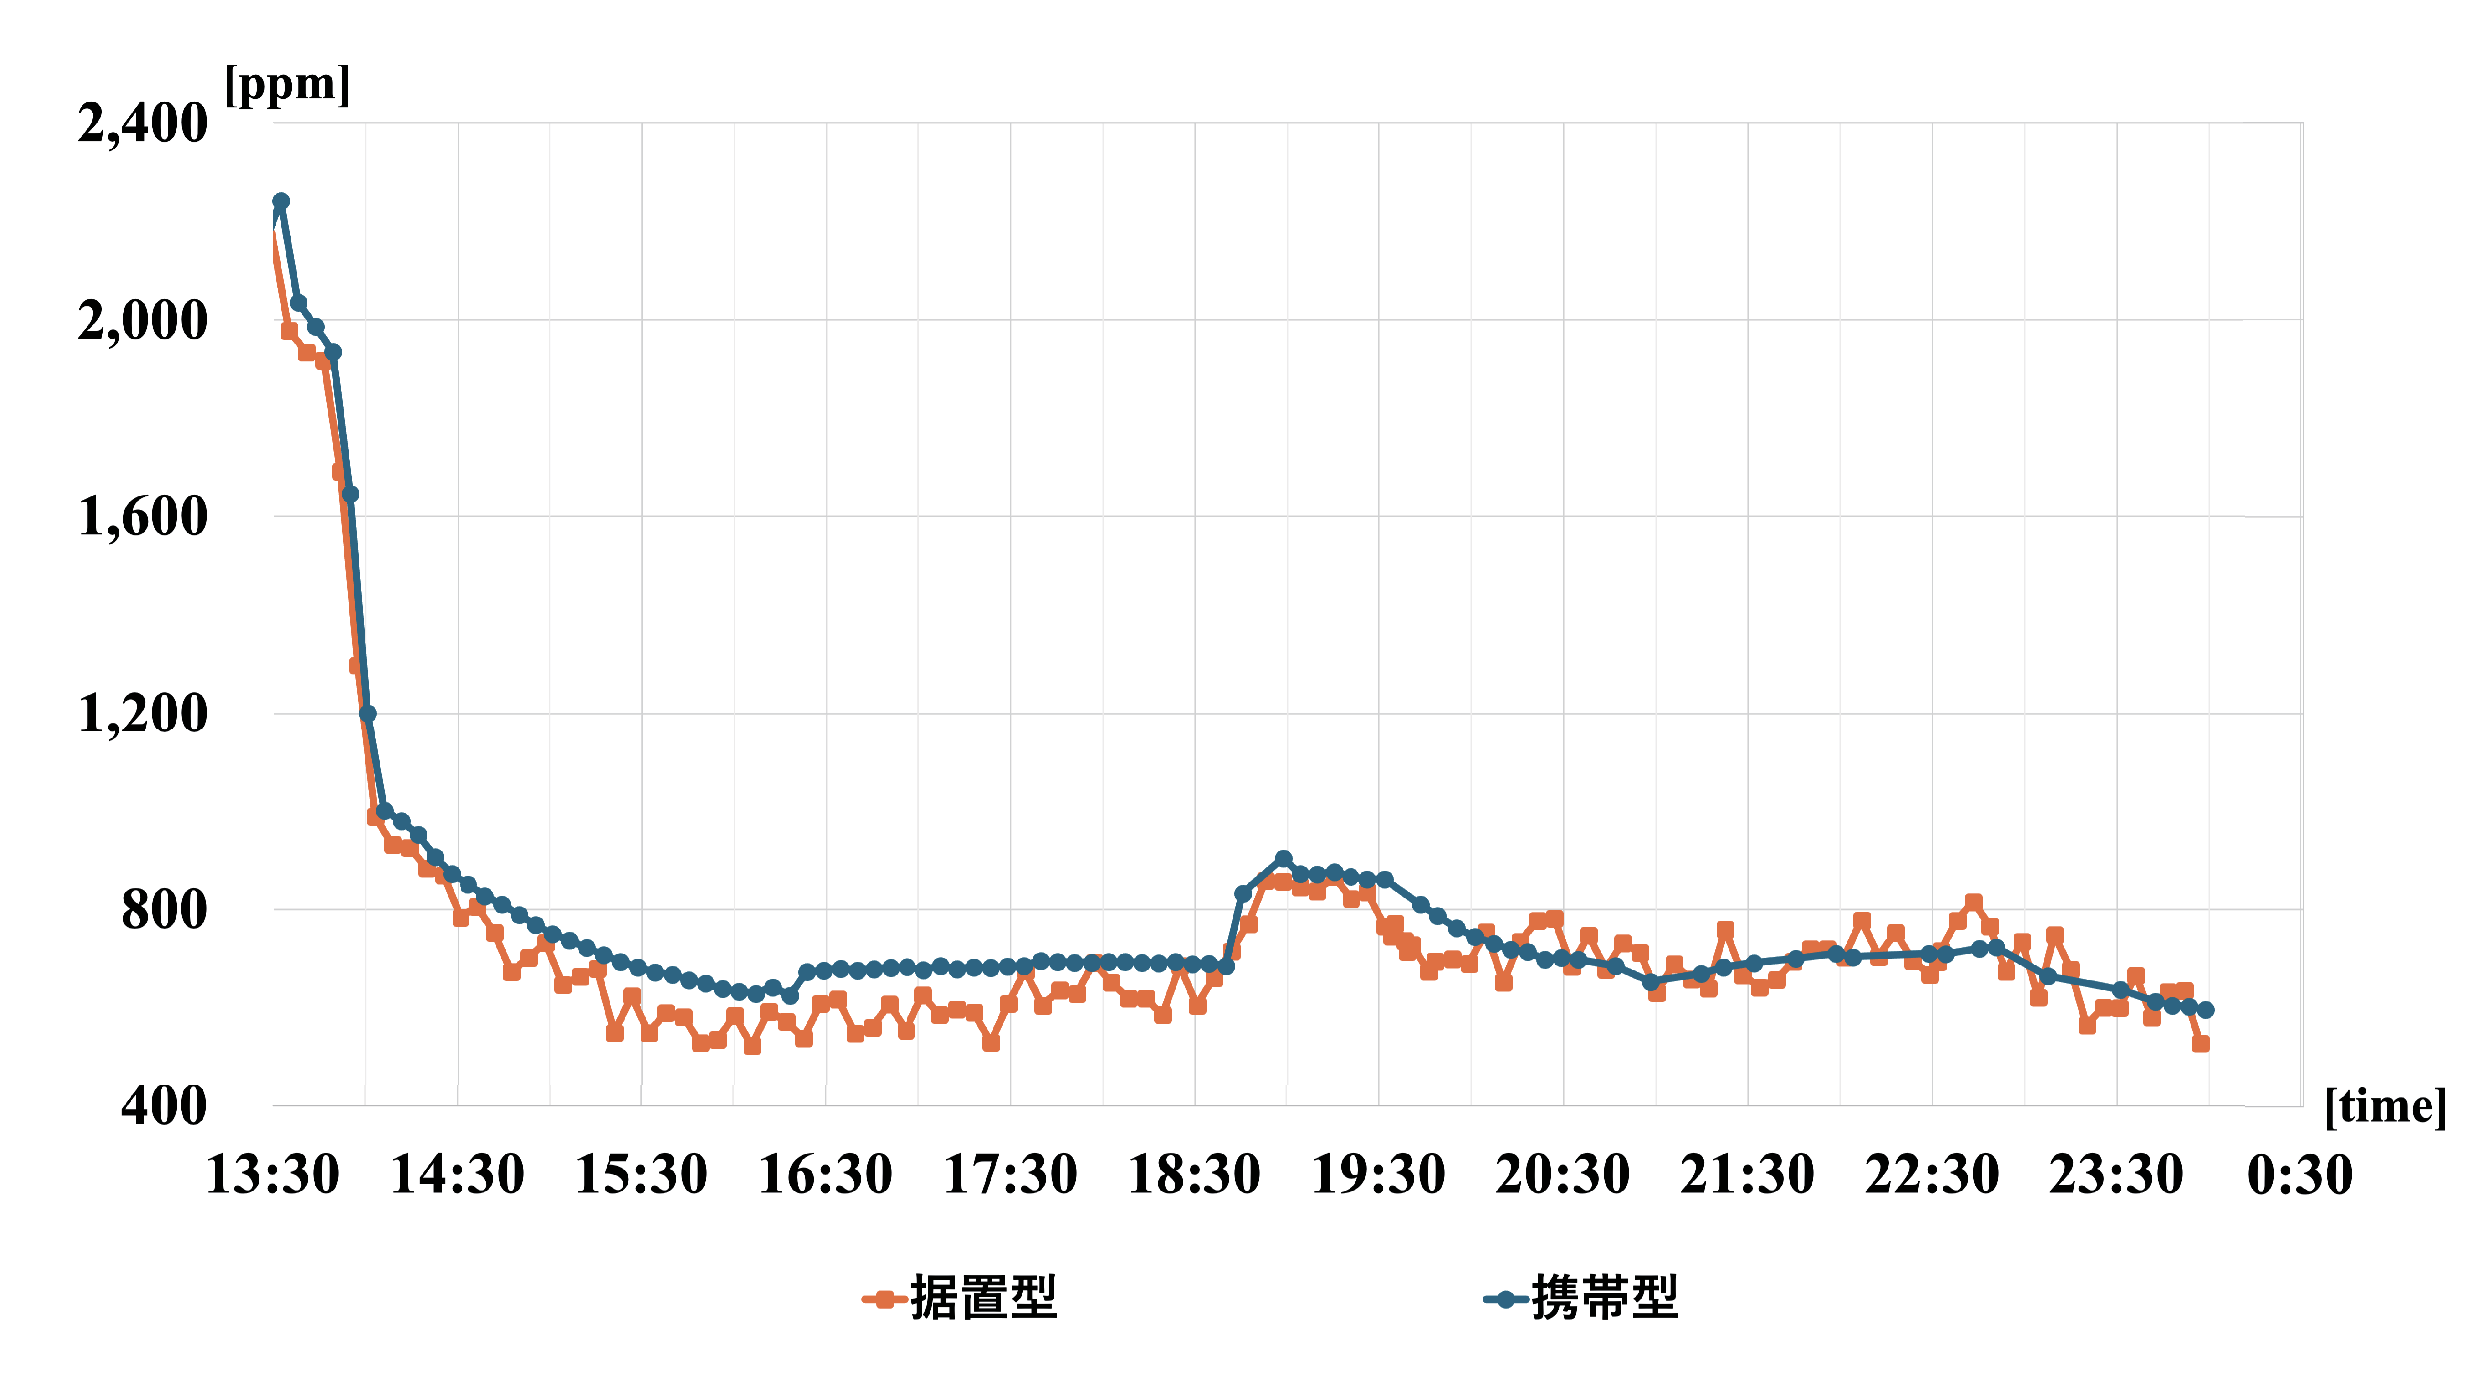
\includegraphics[width=0.9\linewidth]{./figures/センサ比較}
\caption{
据え置き型と携帯型のCO$_2$濃度の比較
}
\label{fig:fixed_vs_portable}
\end{figure}

\section{空間的CO$_2$濃度分布環境における測定結果}
\subsection{ドームハウス内の据え置き型 CO$_2$ 測定機器による測定結果}
据え置き型 CO$_2$ 測定機器を用いてドームハウス内の CO$_2$ 濃度分布を測定した結果を図 \ref{fig:height_co2_comparison} に示す.据え置き型測定機器による測定結果では,階段下から階段上部,さらに 2 階上部へと高さが増加するにつれて,CO$_2$ 濃度が段階的に上昇する傾向が確認された.特に,階段上部および 2 階上部では,階段下部と比較して高い CO$_2$ 濃度が観測されており,ドームハウス内部において CO$_2$ が上部に滞留しやすい空間構造を有していることが示唆される.この結果は,空気の対流や換気経路の影響により,高さ方向に CO$_2$ 濃度の偏りが生じている可能性を示している.


\subsection{ドームハウス内の小型 CO$_2$ 測定デバイスによる測定結果}
次に,本研究で試作した携帯型 CO$_2$ 測定デバイスを用いて,同様にドームハウス内の高さ方向における測定を行った.その結果,小型デバイスにおいても,据え置き型 CO$_2$ 測定機器と同様に,高さの増加に伴って CO$_2$ 濃度が上昇する傾向が確認された.小型デバイスによる測定値は,据え置き型測定機器の測定値と比較して全体的に高い値を示しているが,これはキャリブレーション条件や測定環境の違いによる影響であると考えられる.一方で,階段上部および 2 階上部において CO$_2$ 濃度が高くなるという相対的な変化の傾向は,据え置き型測定機器の結果と概ね一致している.

\subsection{ドームハウス内の据え置き型測定機器との比較評価}

図 \ref{fig:height_co2_comparison} は,据え置き型 CO$_2$ 測定機器および携帯型 CO$_2$ 測定デバイスによる測定結果を,各測定点を 5 点ずつ平均化し,高さ方向に 7 区分して比較したものである.本図より,両者の測定結果は絶対値こそ異なるものの,高さ方向に沿った CO$_2$ 濃度の遷移の仕方が類似していることが分かる.特に,階段下部から階段上部にかけての上昇傾向,および 2 階上部における高濃度領域の検出は,両者で共通して確認された.このことから,小型 CO$_2$ 測定デバイスは,多数の据え置き型測定機器を用いなくても,空間内における CO$_2$ 濃度分布の特徴や,相対的に換気が不十分な領域を把握できる可能性が示された.以上の結果より,本研究で試作した携帯型 CO$_2$ 測定デバイスは,利用者が任意の位置で測定を行うことで,空間内の危険性が高い領域を簡便に察知する手段として有効であると考えられる.

\begin{figure}[H]
\centering
\includegraphics[width=0.9\linewidth]{./figures/赤村比較}
\caption{
各測定点におけるCO$_2$濃度比較
}
\label{fig:height_co2_comparison}
\end{figure}




\section{電車内における CO$_2$ 濃度変化}

本節では,JR 九州 鹿児島本線において実施した電車内測定について,
鳥栖行き普通列車(行き)および門司港行き普通列車(帰り)の
2 つの測定結果を示し,
乗客数の変化,ドア開閉状況,および測定位置の違いが
CO$_2$ 濃度に与える影響について考察する.

\subsection{行き(鳥栖行き普通列車)における測定結果}

行きの測定は,鳥栖行き普通列車において実施した.測定結果を図\ref{fig:densya_iki}にしめす.測定は 1 両目において,進行方向最後部のドア付近に位置し,携帯型 CO$_2$ 測定デバイスを腰部に装着した状態で行った.20 時 32 分に九産大前駅から乗車し,21 時 33 分に鳥栖駅へ到着するまでの区間を対象とした.

測定開始直後(20:32~20:40 頃)は,車内の乗客数が少なく,CO$_2$ 濃度は比較的低い値で推移していた.その後,博多駅(20:47 停車)において多数の乗客が乗車したことにより,発車直後から CO$_2$ 濃度の上昇が確認された.この上昇は,乗客の増加に伴う呼気由来の CO$_2$ 発生量の増加によるものと考えられる.

一方,竹下駅(20:51),笹原駅(20:55),南福岡駅(20:58)以降では,乗客が段階的に降車したことに伴い,CO$_2$ 濃度は徐々に低下する傾向を示した.特に,原田駅(21:17 停車)では,列車の待ち合わせのためドアが長時間開放されており,この区間において CO$_2$ 濃度の顕著な低下が観測された.これは,ドア開放による外気流入が車内換気を大きく促進した結果であると考えられる.

以上より,行きの測定結果からは,乗客数の増減およびドア開閉状況が電車内の CO$_2$ 濃度に直接的な影響を与えることが確認できた.


\begin{figure}[H]
\centering
\includegraphics[width=0.7\linewidth]{./figures/電車比較_行き}
\caption{
電車内のco2濃度変化
}
\label{fig:densya_iki}
\end{figure}



\subsection{帰り(門司港行き普通列車)における測定結果}

帰りの測定は,門司港行き普通列車において実施した.測定結果を図\ref{fig:densya_kaeri}に示す.
測定位置は 9 両目の進行方向先頭側ドア付近とし,21 時 41 分に鳥栖駅から乗車し,22 時 43 分に九産大前駅へ到着するまで測定を行った.乗車時点での車内人数は約 4 名と少なく,発車までの間はドアが開放された状態であった.

測定開始直後は,車内の乗客数が少ないことに加え,ドアが開放されていたため,CO$_2$ 濃度は 500~600 ppm 程度の低い値で安定して推移した.その後,各駅での停車と発進を繰り返す中でも,乗客数の変化が小さい区間ではCO$_2$ 濃度に大きな変動は見られなかった.

一方,博多駅(22:26 停車)では,多くの乗客が乗車したことにより,発車後に CO$_2$ 濃度が急激に上昇する挙動が確認された.さらに,ドア付近で会話を行う乗客が存在した区間では,局所的に CO$_2$ 濃度が高くなる傾向が見られた.その後,香椎駅(22:38 停車)では,乗客の降車およびドア開放が長時間続いたことにより,CO$_2$ 濃度は再び低下した.

このように,帰りの測定結果からは,車内人数が少ない状態ではCO$_2$ 濃度が低く保たれる一方で,主要駅における大量乗車やドア付近での会話といった局所的要因により,短時間で CO$_2$ 濃度が上昇することが確認された.
\begin{figure}[H]
\centering
\includegraphics[width=0.7\linewidth]{./figures/電車比較_帰り}
\caption{
電車内のco2濃度変化
}
\label{fig:densya_kaeri}
\end{figure}
\FloatBarrier

\subsection{ドア付近とドアから離れた位置における CO$_2$ 濃度の比較}

本測定では,電車内における換気状況の位置依存性を評価するため,ドア付近(CS2)およびドアから離れた位置(CS1)の2 箇所において CO$_2$ 濃度の測定を行った.両測定点はいずれも同一車両内に位置しているが,ドア開閉や外気流入の影響の受けやすさが異なる点が特徴である.

行きおよび帰りの測定結果を通して,両測定点の CO$_2$ 濃度は概ね同様の増減傾向を示したものの,濃度の絶対値には明確な差が確認された.特に,多くの時間帯において,ドアから離れた位置(CS1)の CO$_2$ 濃度が,ドア付近(CS2)よりも高くなる傾向が見られた.

例えば,行きの測定においては,博多駅通過後の混雑区間において,CS1 では 1300 ppm を超える値が観測された一方,CS2 ではそれより低い値で推移している.これは,ドア付近では停車時のドア開閉に伴って外気が流入しやすく,局所的な換気が促進されるのに対し,ドアから離れた位置では外気流入の影響を受けにくく,呼気由来の CO$_2$ が滞留しやすいためであると考えられる.

また,各駅停車時に着目すると,
ドア開放直後に CO$_2$ 濃度が低下する挙動は
ドア付近(CS2)でより顕著に現れており,ドアから離れた位置(CS1)では低下量が小さい,あるいは時間遅れを伴って現れる場合があった.この結果は同一車両内であっても換気効果が一様ではなく,位置によって大きく異なることを示している.
以上の結果から,電車内においてはドア付近では比較的換気が行われやすい一方で,ドアから離れた座席付近ではCO$_2$ 濃度が高くなりやすい傾向があることが明らかとなった.本研究で試作した携帯型 CO$_2$ 測定デバイスを用いることで,このような車内の位置による換気状況の違いを利用者自身が把握できる可能性が示された.

\section{省電力性能の評価結果}

本節では,測定機器3および測定機器4において,バッテリ駆動時の稼働時間を測定し,通信方式およびシステム構成の違いが消費電力に与える影響について評価を行う.

先行研究においては,Arduino MKR WiFi 1010,MH-Z19C,BME680,および 1100\,mAh のリチウムポリマバッテリを用いたCO$_2$ 測定機器が試作されており,据え置き型センサを携帯可能とする試みが行われていた.しかし,これらの構成では,Wi-Fi 通信および常時動作に伴う消費電力が大きく,連続稼働時間はおおよそ 6~9 時間程度にとどまることが想定されている.このことから,携帯型 CO$_2$ 測定機器の実用化に向けては,さらなる省電力化が課題であった.


\begin{figure}[H]
\centering
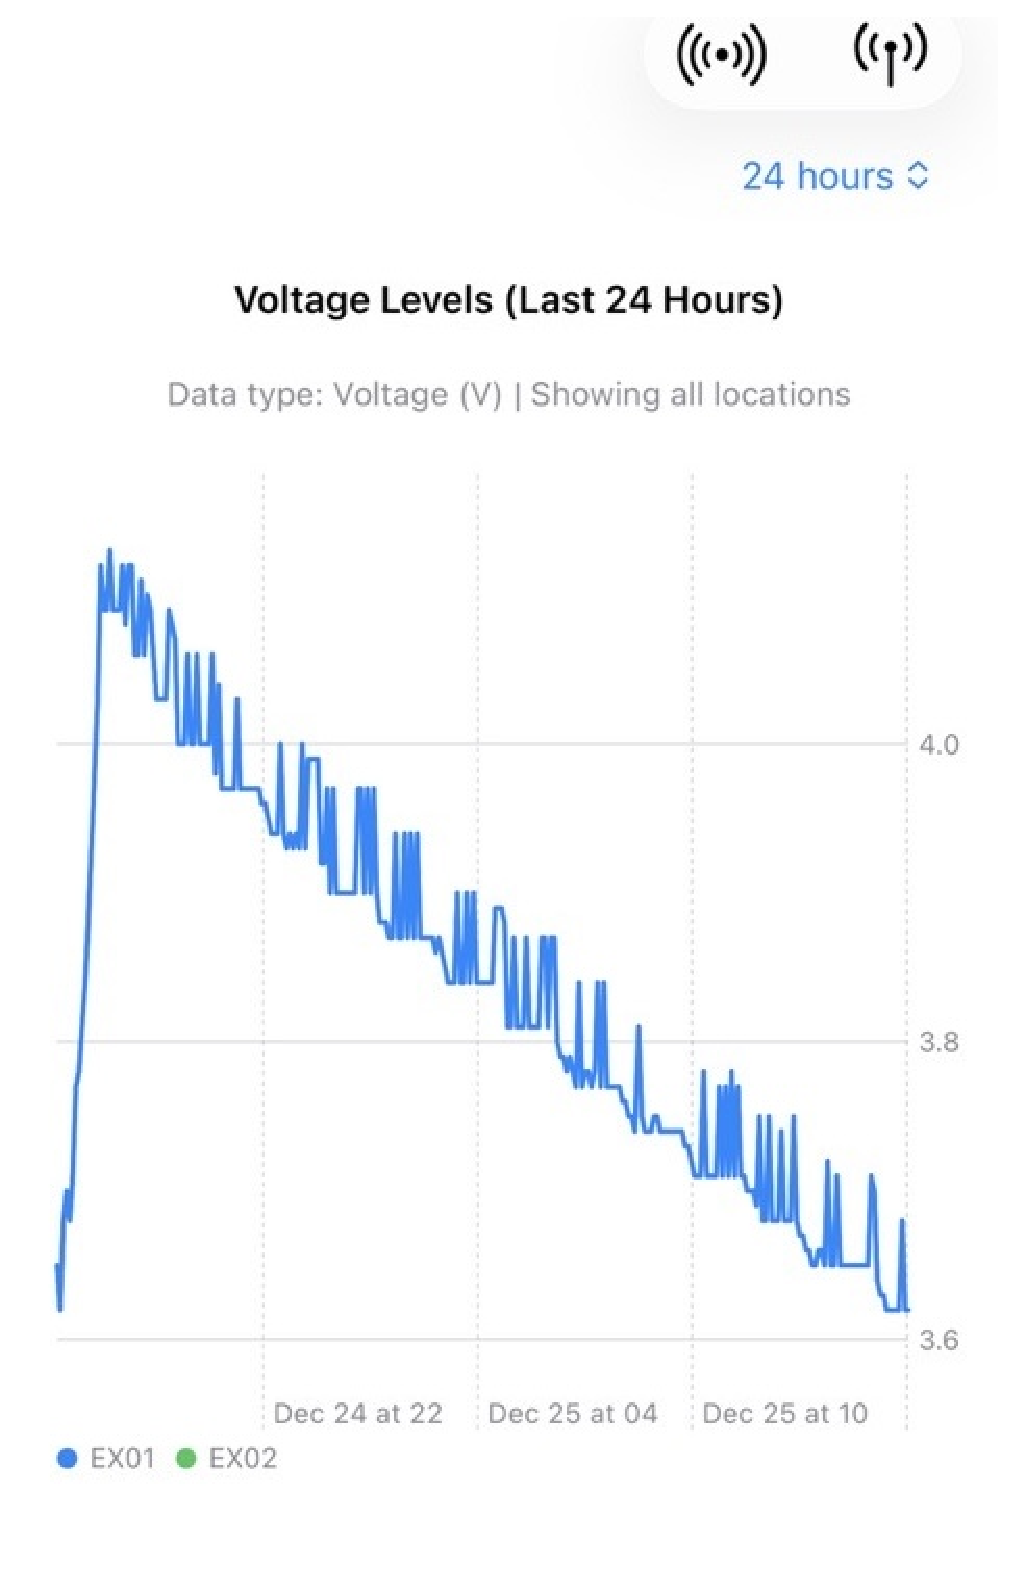
\includegraphics[width=0.5\linewidth]{./figures/voltage-Arduino}
\caption{
測定機器3のバッテリ持続時間
}
\label{fig:voltage-Arduino}
\end{figure}
\FloatBarrier


本研究では,この課題を解決するため,ESP32-C6 を用いたマイクロコントローラ構成と,DeepSleep を活用した周期動作方式を採用し,通信方式の違いによる消費電力の低減効果について検討した.各測定機器には容量 250\,mAh のリチウムポリマバッテリを使用し,測定間隔は 5 分とした.測定時には CO$_2$ 濃度の取得および必要な通信処理を行い,それ以外の時間は ESP32-C6 を DeepSleep 状態へ移行させる構成とした.この条件の下で,バッテリ電圧の時間変化および連続稼働時間を測定した.

LTE 通信モジュール SIM7080G を搭載した測定機器4では,0 時から 15 時までの約 15 時間にわたり連続動作することを確認した.図\ref{fig:voltage} に示すように,動作開始直後は約 4.1\,V 付近であったバッテリ電圧が,時間の経過とともに徐々に低下し,動作終了時には約 3.0\,V まで低下した.この間,設定した測定間隔で測定および通信処理が正常に実行されており,LTE 通信を含む構成においても,DeepSleep を用いた周期動作が実現できていることが確認できた.

\begin{figure}[H]
\centering
\includegraphics[width=0.5\linewidth]{./figures/voltage}
\caption{
測定機器4のバッテリ持続時間
}
\label{fig:voltage}
\end{figure}
\FloatBarrier

一方で,LTE 通信を使用しない測定機器3について評価を行った.測定機器3では,Wi-Fi を用いて測定データを送信する構成であり,LTE 通信モジュールを搭載していない点が特徴である.そのため,セルラ通信に比べて通信時の消費電力を抑えた動作が可能である.その結果,同一条件(測定間隔 5 分,DeepSleep 使用,バッテリ容量 250\,mAh)において,約 56 時間の連続稼働を確認した.

\begin{figure}[H]
\centering
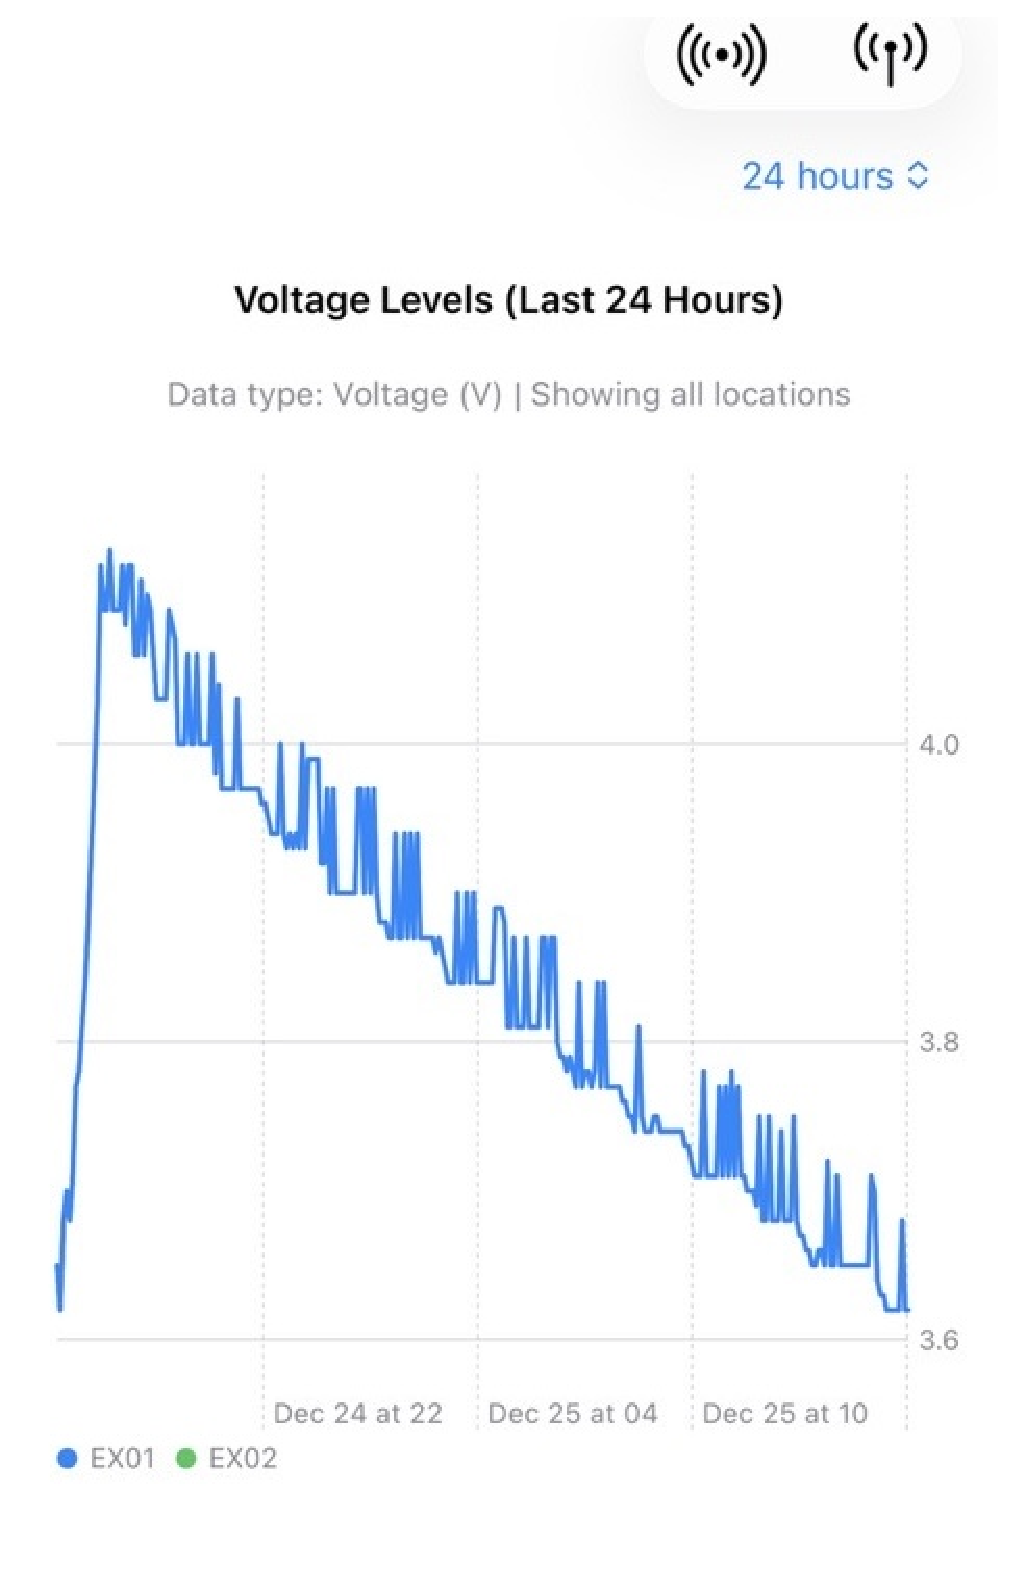
\includegraphics[width=0.5\linewidth]{./figures/voltage-Arduino}
\caption{
測定機器3のバッテリ持続時間
}
\label{fig:voltage-Arduino}
\end{figure}
\FloatBarrier

これらの結果から,先行研究における MH-Z19C を用いた携帯型測定機器と比較して,本研究で提案する測定機器は,バッテリ容量が小さいにもかかわらず,稼働時間を大幅に延長できていることが分かる.特に,Wi-Fi 通信を用いた測定機器3では,先行研究の構成と比較して,約 6 倍以上の連続稼働時間を実現しており,DeepSleep を活用した周期動作設計の有効性が示された.

以上より,本研究で提案する測定機器は,利用目的に応じて通信方式を選択することで,携帯性と稼働時間のバランスを柔軟に調整できる携帯型 CO$_2$ 測定デバイスであることが確認された.


\section{小型化に関する評価}

本節では,本研究で段階的に開発した測定機器1~4について,筐体の小型化の観点から評価を行う.携帯型 CO$_2$ 測定デバイスとして日常生活での利用を想定した場合,測定精度や通信性能に加えて,機器の大きさは携帯性や使用頻度に大きく影響する重要な要素である.

従来,本研究室の先行研究において,据え置き型 CO$_2$ 測定機器が作成され,室内環境における CO$_2$ 濃度の定点観測に用いられてきた.これらの据え置き型測定機器は,長時間にわたる安定した測定が可能であり,空間全体の換気状態を把握する上で有効である一方で,外形寸法が大きく,利用者が身につけて移動しながら測定を行う用途においては,
携帯性の観点から実用が困難であることが,先行研究における課題点として挙げられていた.

そこで本研究では,先行研究で明らかとなった「持ち運びには大きい」という課題を解決することを目的として,小型 CO$_2$ 測定デバイスの開発を行った.
据え置き型測定機器の測定精度や測定手法を踏襲しつつ,日常生活のさまざまな環境において利用者が携帯可能なサイズを実現することを目標とし,小型化を重視した設計を行った.

表\ref{tab:size_comparison}に,据え置き型測定機器および測定機器1~4の外形寸法と体積(外形面積)の比較を示す.据え置き型測定機器は外形寸法が約 73\,mm $\times$ 65\,mm,外形面積が約 4,745\,mm$^2$ であり,携帯型として使用するには大きいことが分かる.これに対し,本研究で試作した測定機器はいずれも,据え置き型測定機器と比較して大幅な小型化が達成されている.

\begin{table}[htbp]
\centering
\caption{据え置き型測定機器および測定機器1~4の外形寸法と体積の比較}
\label{tab:size_comparison}
\begin{tabular}{|l|r|r|}
\hline
測定機器 & 外形寸法 [mm] & 体積 [mm$^2$] \\ \hline \hline
据え置き型測定機器 & 73 $\times$ 65 & 4,745 \\ \hline
測定機器1 & 40 $\times$ 60 & 2,400 \\ \hline
測定機器2 & 50 $\times$ 70 & 3,500 \\ \hline
測定機器3 & 30 $\times$ 40 & 1,200 \\ \hline
測定機器4 & 35 $\times$ 55 & 1,925 \\ \hline
\end{tabular}
\end{table}

測定機器1は,ESP32-C6,SCD41,プッシュボタンおよびリチウムポリマバッテリを用いた最小構成の測定機器であり,外形寸法は約 40\,mm $\times$ 60\,mm であった.本機器は機能確認を主目的として作成したため,部品配置の最適化や筐体サイズの削減は行っておらず,比較的余裕のある寸法となっている.しかしながら,据え置き型測定機器と比較すると,外形面積は約 50\% 程度に抑えられており,携帯型測定機器としての可能性を示す結果である.

測定機器2では,測定機器1の構成を維持したまま,利用者への視覚的フィードバックを目的として LED を追加した.その結果,外形寸法は約 50\,mm $\times$ 70\,mm となり,測定機器1と比較してやや大型化している.これは機能追加を優先した設計によるものであり,試作段階における仕様上の選択である.それでもなお,据え置き型測定機器と比較すると外形面積は小さく,携帯型測定機器としての基本的な要件は満たしている.

測定機器3では,測定機器2で確認された機能を維持しつつ,携帯性の向上を目的として筐体の小型化を行った.部品配置を見直し,ESP32-C6 の表面および裏面の両方に部品を実装する構成とすることで,外形寸法は約 30\,mm $\times$ 40\,mm まで縮小された.測定機器1と比較すると,外形面積は約 2,400\,mm$^2$ から約 1,200\,mm$^2$ へと減少しており,約 50\% の削減が達成されている.また,据え置き型測定機器と比較すると,外形面積は約 75\% 削減されており,本研究の目的である携帯性の向上が大きく達成されたことが分かる.

さらに,測定機器4では,測定機器3で達成した小型化を意識しつつ,LTE 通信モジュールである SIM7080G を新たに搭載した.通信機能の追加により構成は複雑化したものの,外形寸法は約 35\,mm $\times$ 55\,mm に抑えられている.

測定機器2と比較すると,外形面積は約 3,500\,mm$^2$ から約 1,925\,mm$^2$ へと減少しており,約 45\% の小型化が実現されている.これは,通信機能を追加しながらも,部品配置の最適化によって筐体の縮小が可能であったことを示している.また,据え置き型測定機器と比較すると,外形面積は約 4,745\,mm$^2$ から約 1925\,mm$^2$ へと減少しており,約 60\% の小型化が達成されている.この結果から,LTE 通信を備えた構成であっても,据え置き型測定機器では困難であった携帯性を確保できることが明らかとなった.

以上の結果から,本研究では据え置き型 CO$_2$ 測定機器の課題であった大型化という問題に対し,ESP 系マイクロコントローラを用いた段階的な設計改良を行うことで,機能追加と小型化の両立を実現してきたといえる.特に,測定機器3および測定機器4では,,ネックレスや腰部への装着といった利用形態にも適した携帯型 CO$_2$ 測定デバイスであると評価できる.







